\documentclass[a4paper,12pt]{report}
\usepackage[utf8]{inputenc}
\usepackage{lmodern}
\usepackage{enumitem}
\usepackage{titlesec}
\usepackage{graphicx}
\usepackage{tabularx}
\usepackage{amsmath}
\usepackage{amssymb}
\usepackage[italian]{babel}
\usepackage[margin=2cm]{geometry}

\title{Progetto 20070703 (P.20070703) - DormoDaTe}
\author{Sebastiano Deodati}

\titleformat{\chapter}[display]{\normalfont\huge\bfseries}{}{0pt}{\Huge}

\begin{document}
  \maketitle
  \tableofcontents

  \chapter{Dati di interesse e funzionalità richieste}
    \begin{enumerate}[label*=\arabic*.]
      \item Utente:
        \begin{enumerate}[label*=\arabic*.]
          \item Nickname (univoco)
          \item Nome
          \item Cognome
          \item Sesso
          \item Data di nascita
          \item Città di residenza (req. 2)
          \item Ospitalità offerta (req. 3)
        \end{enumerate}
      \item Città:
        \begin{enumerate}[label*=\arabic*.]
          \item Nome
          \item Provincia
        \end{enumerate}
      \item Casa:
        \begin{enumerate}[label*=\arabic*.]
          \item Indirizzo (req. 4)
          \item Distanza (mt) dal centro città
          \item Distanza (mt) dalla stazione autobus/metro/treno più vicina
          \item Adulti residenti
          \item Bambini residenti
          \item Camere (req. 5)
        \end{enumerate}
      \item Indirizzo:
        \begin{enumerate}[label*=\arabic*.]
          \item Via/Piazza
          \item Numero civico
          \item Città (req. 2)
        \end{enumerate}
      \item Camera:
        \begin{enumerate}[label*=\arabic*.]
          \item Ubicazione (req. 3)
          \item Posti letto (req. 6)
          \item Eventuali periodi di indisponibilità
        \end{enumerate}
      \newpage
      \item Posto letto:
        \begin{enumerate}[label*=\arabic*.]
          \item Ubicazione (req. 5)
          \item Tipo (letto singolo, letto matrimoniale, divano letto)
          \item Eventuali periodi di indisponibilità
        \end{enumerate}
      \item Prenotazione:
        \begin{enumerate}[label*=\arabic*.]
          \item Richiedente (req. 1)
          \item Eventuali accompagnatori (req. 1)
          \item Scelta dei posti letto (req. 6)
          \item Periodo di prenotazione
          \item Stato (in attesa, accettata, rifiutata)
            \begin{enumerate}[label*=\arabic*.]
              \item Motivazione del rifiuto (se rifiutata)
            \end{enumerate}
          \item Istante di prenotazione (per controllo su feedback obbligatori)
        \end{enumerate}
      \item Feedback:
        \begin{enumerate}[label*=\arabic*.]
          \item Prenotazione di riferimento (req. 7)
          \item Feedback di tutti gli ospiti (voto da 0 a 5)
          \item Feedback dell'ospitante sugli ospiti (facoltativo)
        \end{enumerate}
      \item Funzionalità richieste:
        \begin{enumerate}[label*=\arabic*.]
          \item Il sistema deve consentire a tutti gli iscritti di aggiornare in qualunque momento le informazioni circa la sua disponibilità ad ospitare persone, per ogni sistemazione, specificando date in cui una data sistemazione non è disponibile
          \item I viaggiatori che desiderano organizzare un viaggio usufruendo del servizio devono poter interrogare il sistema per ottenere l’insieme di tutti gli iscritti della città desiderata che sono disposti a ricevere ospiti nel periodo richiesto e hanno, per le date richieste, posti sufficienti disponibili
          \item Data una richiesta di prenotazione, il relativo ospitante deve poter liberamente accettare o rifiutare la richiesta, in quest'ultimo caso specificando il motivo
          \item Al termine di un periodo di ospitazione, l'ospitante deve poter esprimere un feedback (voto da 0 a 5) sui suoi ospiti, mentre gli ospiti devono essere costretti ad esprimere un feedback sull'ospitante, impedendogli di effettuare un'altra prenotazione finché non avranno espresso il loro feedback
        \end{enumerate}
    \end{enumerate}
    \chapter{Diagramma ER}
      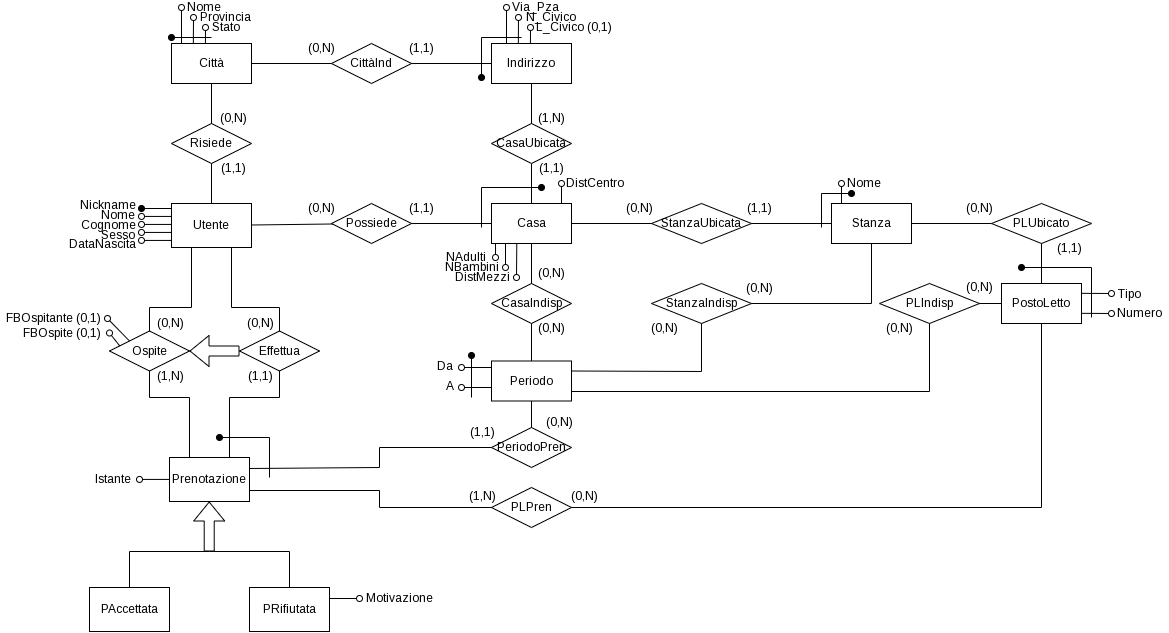
\includegraphics[width=1\textwidth]{er.png}
    \chapter{Dizionario dei dati}
      Entità Utente: \\
      \begin{tabular}{|c|c|c|}
        \hline Attributo & Tipo & Note \\
        \hline Nickname & stringa & \\
        \hline Nome & Stringa & \\
        \hline Cognome & Stringa & \\
        \hline Sesso & \{'M', 'F'\} & \\
        \hline Nascita & dataora & \\
        \hline
      \end{tabular} \\
      \vspace{24pt} \\
      Entità Città: \\
      \begin{tabular}{|c|c|c|}
        \hline Attributo & Tipo & Note \\
        \hline Nome & stringa & \\
        \hline Provincia & stringa & \\
        \hline Stato & stringa & \\
        \hline
      \end{tabular} \\
      \vspace{24pt} \\
      Entità Indirizzo: \\
      \begin{tabular}{|c|c|c|}
        \hline Attributo & Tipo & Note \\
        \hline Via\_Pza & stringa & \\
        \hline N\_Civico & intero \(\geq 0\) & 0 indica SNC \\
        \hline L\_Civico(0,1) & lettera & Lettera del numero civico (opzionale) \\
        \hline
      \end{tabular} \\
      \vspace{24pt} \\
      Entità Casa: \\
      \begin{tabular}{|c|c|c|}
        \hline Attributo & Tipo & Note \\
        \hline DistMezzi & intero \(> 0\) & Distanza in metri dalla stazione dei trasporti pubblici più vicina \\
        \hline DistCentro & intero \(> 0\) & Distanza in metri dal centro città \\
        \hline NAdulti & intero \(\geq 0\) & Adulti residenti \\
        \hline NBambini & intero \(\geq 0\) & Bambini residenti \\
        \hline
      \end{tabular} \\
      \vspace{24pt} \\
      Entità Periodo: \\
      \begin{tabular}{|c|c|c|}
        \hline Attributo & Tipo & Note \\
        \hline Da & dataora & Inizio del periodo di tempo \\
        \hline A & dataora & Fine del periodo di tempo \\
        \hline
      \end{tabular} \\
      \newpage
      Entità Stanza: \\
      \begin{tabular}{|c|c|c|}
        \hline Attributo & Tipo & Note \\
        \hline Nome & stringa & \\
        \hline
      \end{tabular} \\
      \vspace{24pt} \\
      Entità PostoLetto: \\
      \begin{tabular}{|c|p{0.4\textwidth}|p{0.4\textwidth}|}
        \hline Attributo & Tipo & Note \\
        \hline Numero & intero \(\geq 0\) & Un numero incrementale per identificare i posti letto dello stesso tipo in una stanza \\
        \hline Tipo & \{'Letto singolo', 'Letto matrimoniale', 'Divano letto'\} & Il tipo identifica anche il numero di posti \\
        \hline
      \end{tabular} \\
      \vspace{24pt} \\
      Entità Prenotazione: \\
      \begin{tabular}{|c|p{0.4\textwidth}|p{0.4\textwidth}|}
        \hline Attributo & Tipo & Note \\
        \hline Istante & dataora & Istante della prenotazione, utilizzato per impedire agli utenti di effettuare prenotazioni in mancanza di feedback relativi a vecchie prenotazioni \\
        \hline
      \end{tabular} \\
      \vspace{24pt} \\
      Entità PRifiutata: \\
      \begin{tabular}{|c|c|c|}
        \hline Attributo & Tipo & Note \\
        \hline Motivazione & stringa & Motivo del rifiuto \\
        \hline
      \end{tabular} \\
      \vspace{24pt} \\
      Relazione Ospite: \\
      \begin{tabular}{|c|c|c|}
        \hline Attributo & Tipo & Note \\
        \hline FBOspite(0,1) & intero[0,5] & Feedback espresso dall'ospitante sull'ospite \\
        \hline FBOspitante(0,1) & intero[0,5] & Feedback espresso dall'ospite sull'ospitante \\
        \hline
      \end{tabular} \\

      \vspace{24pt}
      \large Vincoli esterni: \\
      \normalsize
      V.Indirizzo.lettera: $\forall i \;\; Indirizzo(i) \; \wedge \; NCivico(i, 0) \; \rightarrow \; \neg \exists \; l \;\; lettera(l) \; \wedge \; LCivico(i, l)$ \\
      V.Periodo.nonneg: $\forall p,i,f \;\; Periodo(p) \; \wedge \; Da(p, i) \; \wedge A(p, f) \; \rightarrow \; i \; \leq \; f$ \\
      V.Utente.fb\_obbligatorio: $\forall u,p,i \;\; Utente(u) \; \wedge \; Prenotazione(p) \; \wedge \; Istante(p, i) \; \wedge \; Ospite(u, p) \; \rightarrow \forall p',i' \; [Prenotazione(p') \; \wedge \; Istante(p', i') \; \wedge \; i' < i] \; \rightarrow \; \exists \; f \; "intero[0,5]"(f) \; \wedge \; FBOspitante(u, p', f)$ \\
    \chapter{UML}
      \begin{center}
        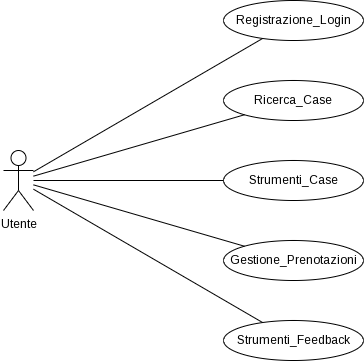
\includegraphics{uml.png}
      \end{center}
    \chapter{Specifiche degli use-case}
      \section*{Specifiche use-case Registrazione\_Login}
        \textbf{Registra}(nickname: stringa, nome: stringa, cognome: stringa, sesso: \{'M', 'F'\}, nascita: data, residenza: Citta) : Utente \\
        \hspace*{1cm} precondizioni: $\neg \exists u \;\; Utente(u) \; \wedge \; Nickname(u, nickname)$ \\
        \hspace*{1cm} postcondizioni: \\
        \hspace*{2cm} modifica al livello estensionale dei dati: \\
        \hspace*{3cm} nuovi elementi del dominio di interpretazione: u \\
        \hspace*{3cm} nuove ennuple di predicati: \\
        \hspace*{4cm} Utente(u) \\
        \hspace*{4cm} Nickname(u, nickname) \\
        \hspace*{4cm} Nome(u, nome) \\
        \hspace*{4cm} Cognome(u, cognome) \\
        \hspace*{4cm} Sesso(u, sesso) \\
        \hspace*{4cm} DataNascita(u, nascita) \\
        \hspace*{4cm} Risiede(u, residenza) \\
        \hspace*{2cm} valore di ritorno: $result = u$ \\ \\

        \hspace*{-1cm}
        \textbf{Login}(nickname: Stringa) : Utente \\
        \hspace*{1cm} precondizioni: $\exists u \;\; Utente(u) \; \wedge \; Nickname(u, nickname)$ \\
        \hspace*{1cm} postcondizioni: \\
        \hspace*{2cm} modifica al livello estensionale dei dati: nessuna \\
        \hspace*{2cm} valore di ritorno: \\
        \hspace*{3cm} Sia $u$ t.c. $Utente(u) \; \wedge \; Nickname(u, nickname)$ \\
        \hspace*{3cm} $result = u$ \\ \\

      \newpage

      \section*{Specifiche use-case Ricerca\_Case}
        \textbf{Cerca}(citta: Citta, p: Periodo, nposti: intero $>$ 0) : Casa(0,N) \\
        \hspace*{1cm} precondizioni: nessuna \\
        \hspace*{1cm} postcondizioni: \\
        \hspace*{2cm} modifica al livello estensionale dei dati: nessuna \\
        \hspace*{2cm} valore di ritorno: \\
        \hspace*{3cm} Sia $C_{citta}$ = \{$c \, | \, Casa(c) \, \wedge \, [\exists i \, Indirizzo(i) \, \wedge \, CasaUbicata(c, i) \, \wedge \, CittaInd(citta, i)]$\} \\
        \hspace*{3cm} sia $C_{ok}$ = \{$c \, \in \, C_{citta} \, | \, "Operazioni\_Case".Posti\_disponibili(c, p) \, > \, nposti$\} \\
        \hspace*{3cm} $result = C_{ok}$ \\ \\

      \section*{Specifiche use-case Strumenti\_Case}
        \textbf{PL\_disponibile}(pl: PostoLetto, p: Periodo) : booleano \\
        \hspace*{1cm} precondizioni: nessuna \\
        \hspace*{1cm} postcondizioni: \\
        \hspace*{2cm} modifica al livello estensionale dei dati: nessuna \\
        \hspace*{2cm} valore di ritorno: \\
        \hspace*{3cm} $result = [\exists c, s \, PLUbicato(p, s) \, \wedge \, StanzaUbicata(s, c)] \\
        \hspace*{4cm} \wedge \, [\neg \exists pr,p' \, Prenotazione(pr) \, \wedge \, PLPren(pr, p') \, \wedge p \cap p' \neq \varnothing] \\
        \hspace*{4cm} \wedge \, [\neg \exists i,j,k \, PLIndisp(p, i) \, \wedge \, StanzaIndisp(s, j) \, \wedge \, CasaIndisp(c, k) \\
        \hspace*{5cm} \wedge \, (i \cup j \cup k) \cap p \neq \varnothing]$ \\ \\

        \hspace*{-1cm}
        \textbf{Posti\_disponibili}(c: Casa, p: Periodo) : intero $\geq$ 0 \\
        \hspace*{1cm} precondizioni: nessuna \\
        \hspace*{1cm} postcondizioni: \\
        \hspace*{2cm} modifica al livello estensionale dei dati: nessuna \\
        \hspace*{2cm} valore di ritorno: \\
        \hspace*{3cm} Sia $P_{L1}$ = \{$pl \, | \, PostoLetto(pl) \, \wedge \, Tipo(pl, 'Letto singolo') \\
        \hspace*{4cm} \wedge \, "Strumenti\_Case".PL\_disponibile(pl, p) = vero$\} \\
        \hspace*{3cm} Sia $P_{L2}$ = = \{$pl \, | \, PostoLetto(pl) \, \wedge \, \neg(Tipo(pl, 'Letto singolo')) \\
        \hspace*{4cm} \wedge \, "Strumenti\_Case".PL\_disponibile(pl, p) = vero$\} \\
        \hspace*{3cm} $result = |P_{L1}| + 2*|P_{L2}|$ \\ \\

        \newpage

        \hspace*{-1cm}
        \textbf{Registra\_Casa}(u: Utente, indirizzo: Indirizzo, distCentro: intero $\geq$ 0, distMezzi: intero $\geq$ 0, nAdulti: intero $\geq$ 0, nBambini: intero $\geq$ 0) : Casa \\
        \hspace*{1cm} precondizioni: nessuna \\
        \hspace*{1cm} postcondizioni: \\
        \hspace*{2cm} modifica al livello estensionale dei dati: \\
        \hspace*{3cm} nuovi elementi del dominio di interpretazione: c \\
        \hspace*{3cm} nuove ennuple di predicati: \\
        \hspace*{4cm} Casa(c) \\
        \hspace*{4cm} DistCentro(c, distCentro) \\
        \hspace*{4cm} DistMezzi(c, distMezzi) \\
        \hspace*{4cm} NAdulti(c, nAdulti) \\
        \hspace*{4cm} NBambini(c, nBambini) \\
        \hspace*{4cm} Possiede(u, c) \\
        \hspace*{4cm} CasaUbicata(c, indirizzo) \\
        \hspace*{2cm} valore di ritorno: $result = c$ \\ \\

        \hspace*{-1cm}
        \textbf{Registra\_Stanza}(u: Utente, c: Casa, nome: stringa) : Stanza \\
        \hspace*{1cm} precondizioni: nessuna \\
        \hspace*{1cm} postcondizioni: \\
        \hspace*{2cm} modifica al livello estensionale dei dati: \\
        \hspace*{3cm} nuovi elementi del dominio di interpretazione: s \\
        \hspace*{3cm} nuove ennuple di predicati: \\
        \hspace*{4cm} Stanza(s) \\
        \hspace*{4cm} Nome(s, nome) \\
        \hspace*{4cm} StanzaUbicata(s, c) \\
        \hspace*{2cm} valore di ritorno: $result = s$ \\ \\

        \hspace*{-1cm}
        \textbf{Registra\_PostoLetto}(u: Utente, s: Stanza, tipo: \{'Letto singolo', 'Letto matrimoniale', 'Divano letto'\}, n: intero $\geq$ 0) : PostoLetto \\
        \hspace*{1cm} precondizioni: $\neg \exists p \; PostoLetto(p) \; \wedge \; PLUbicato(p, s) \; \wedge \; Tipo(p, tipo) \; \wedge \; Numero(p, n)$ \\
        \hspace*{1cm} postcondizioni: \\
        \hspace*{2cm} modifica al livello estensionale dei dati: \\
        \hspace*{3cm} nuovi elementi del dominio di interpretazione: p \\
        \hspace*{3cm} nuove ennuple di predicati: \\
        \hspace*{4cm} PostoLetto(p) \\
        \hspace*{4cm} Tipo(p, tipo) \\
        \hspace*{4cm} Numero(p, n) \\
        \hspace*{4cm} PLUbicato(p, s) \\
        \hspace*{2cm} valore di ritorno: $result = p$ \\ \\

        \newpage

        \hspace*{-1cm}
        \textbf{Indisponibilita\_Casa}(c: Casa, p: Periodo) \\
        \hspace*{1cm} precondizioni: $\neg CasaIndisp(c, p)$ \\
        \hspace*{1cm} postcondizioni: \\
        \hspace*{2cm} modifica al livello estensionale dei dati: \\
        \hspace*{3cm} dominio di interpretazione: invariato \\
        \hspace*{3cm} nuove ennuple di predicati: CasaIndisp(c, p) \\
        \hspace*{2cm} valore di ritorno: nessuno \\ \\

        \hspace*{-1cm}
        \textbf{Indisponibilita\_Stanza}(s: Stanza, p: Periodo) \\
        \hspace*{1cm} precondizioni: $\neg StanzaIndisp(s, p)$ \\
        \hspace*{1cm} postcondizioni: \\
        \hspace*{2cm} modifica al livello estensionale dei dati: \\
        \hspace*{3cm} dominio di interpretazione: invariato \\
        \hspace*{3cm} nuove ennuple di predicati: StanzaIndisp(s, p) \\
        \hspace*{2cm} valore di ritorno: nessuno \\ \\

        \hspace*{-1cm}
        \textbf{Indisponibilita\_PL}(pl: PostoLetto, p: Periodo) \\
        \hspace*{1cm} precondizioni: $\neg PLIndisp(pl, p)$ \\
        \hspace*{1cm} postcondizioni: \\
        \hspace*{2cm} modifica al livello estensionale dei dati: \\
        \hspace*{3cm} dominio di interpretazione: invariato \\
        \hspace*{3cm} nuove ennuple di predicati: PLIndisp(pl, p) \\
        \hspace*{2cm} valore di ritorno: nessuno \\ \\

      \section*{Specifiche use-case Gestione\_Prenotazioni}
        \textbf{Prenota}(u: Utente, A: Utente(0,N), PL: PostoLetto(1,N), p: Periodo) : Prenotazione \\
        \hspace*{1cm} precondizioni: \\
        \hspace*{2cm}$\exists c \; Casa(c) \; \wedge \; [\forall pl \in PL \; \exists s \; PLUbicato(pl, s) \wedge StanzaUbicata(s, c)]$ \\
        \hspace*{2cm}$"Strumenti\_Case".PL\_disponibile(pl, p) \, \forall pl \in PL$ \\
        \hspace*{1cm} postcondizioni: \\
        \hspace*{2cm} modifica al livello estensionale dei dati: \\
        \hspace*{3cm} nuovi elementi del dominio di interpretazione: pr \\
        \hspace*{3cm} nuove ennuple di predicati: \\
        \hspace*{4cm} Prenotazione(pr) \\
        \hspace*{4cm} Istante(pr, \textit{adesso}) \\
        \hspace*{4cm} Effettua(u, pr) \\
        \hspace*{4cm} Ospite(u, pr) \\
        \hspace*{4cm} Ospite(a, pr) $\forall a \in A$ \\
        \hspace*{4cm} PeriodoPren(p, pr) \\
        \hspace*{4cm} PLPren(pl, pr) $\forall pl \in PL$ \\
        \hspace*{2cm} valore di ritorno: $result = pr$ \\ \\

        \hspace*{-1cm}
        \textbf{Accetta\_Prenotazione}(h: Utente, p: Prenotazione) \\
        \hspace*{1cm} precondizioni: $\exists pl, s, c \, PLPRen(pl, p) \wedge PLUbicato(pl, s) \wedge StanzaUbicata(s, c) \wedge Possiede(h, c)$ \\
        \hspace*{1cm} postcondizioni: \\
        \hspace*{2cm} modifica al livello estensionale dei dati: \\
        \hspace*{3cm} dominio di interpretazione: invariato \\
        \hspace*{3cm} nuove ennuple di predicati: PAccettata(p) \\
        \hspace*{2cm} valore di ritorno: nessuno \\ \\

        \hspace*{-1cm}
        \textbf{Rifiuta\_Prenotazione}(h: Utente, p: Prenotazione, motivo: stringa) \\
        \hspace*{1cm} precondizioni: $\exists pl, s, c \, PLPRen(pl, p) \wedge PLUbicato(pl, s) \wedge StanzaUbicata(s, c) \wedge Possiede(h, c)$ \\
        \hspace*{1cm} postcondizioni: \\
        \hspace*{2cm} modifica al livello estensionale dei dati: \\
        \hspace*{3cm} dominio di interpretazione: invariato \\
        \hspace*{3cm} nuove ennuple di predicati: \\
        \hspace*{4cm} PRifiutata(p) \\
        \hspace*{4cm} Motivazione(p, motivo) \\
        \hspace*{2cm} valore di ritorno: nessuno \\ \\

        \hspace*{-1cm}
        \textbf{Annulla\_Prenotazione}(u: Utente, p: Prenotazione) \\
        \hspace*{1cm} precondizioni: $Effettua(u, p) \; \wedge \; \neg PRifiutata(p) \\
        \hspace*{2cm} \wedge \; \neg \exists per, i \, [PeriodoPren(per, p) \wedge Da(per, i) \wedge i \geq \textit{adesso}]$ \\
        \hspace*{1cm} postcondizioni: \\
        \hspace*{2cm} modifica al livello estensionale dei dati: \\
        \hspace*{3cm} elementi del dominio di interpretazione che non esistono più: p \\
        \hspace*{3cm} ennuple di predicati che non valgono più: \\
        \hspace*{4cm} Prenotazione(p) \\
        \hspace*{4cm} PAccettata(p) \\
        \hspace*{2cm} valore di ritorno: nessuno \\ \\

      \section*{Specifiche use-case Strumenti\_Feedback}
        \textbf{Valuta\_Ospitante}(u: Utente, p: PAccettata, voto: intero [0,5]) \\
        \hspace*{1cm} precondizioni: $Ospite(u, p) \; \wedge \; \exists per, f \, [PeriodoPren(per, p) \wedge A(per, f) \wedge f \leq \textit{adesso}]$ \\
        \hspace*{1cm} postcondizioni: \\
        \hspace*{2cm} modifica al livello estensionale dei dati: \\
        \hspace*{3cm} dominio di interpretazione: invariato \\
        \hspace*{3cm} nuove ennuple di predicati: FBOspitante(u, p, voto) \\
        \hspace*{2cm} valore di ritorno: nessuno \\ \\

        \newpage

        \hspace*{-1cm}
        \textbf{Valuta\_Ospite}(h: Utente, o: Utente, p: PAccettata, voto: intero [0,5]) \\
        \hspace*{1cm} precondizioni: $Ospite(o, p) \; \wedge \; \exists pl, s, c \\
        \hspace*{2cm} [PLPRen(pl, p) \wedge PLUbicato(pl, s) \wedge StanzaUbicata(s, c) \wedge Possiede(h, c)] \\
        \hspace*{3cm} \wedge \; \exists per, f \, [PeriodoPren(per, p) \wedge A(per, f) \wedge f \leq \textit{adesso}]$ \\
        \hspace*{1cm} postcondizioni: \\
        \hspace*{2cm} modifica al livello estensionale dei dati: \\
        \hspace*{3cm} dominio di interpretazione: invariato \\
        \hspace*{3cm} nuove ennuple di predicati: FBOspite(o, p, voto) \\
        \hspace*{2cm} valore di ritorno: nessuno \\ \\

        \hspace*{-1cm}
        \textbf{Feedback\_Ospitante}(h: Utente) : intero[0,5](0,N) \\
        \hspace*{1cm} precondizioni: nessuna \\
        \hspace*{1cm} postcondizioni: \\
        \hspace*{2cm} modifica al livello estensionale dei dati: nessuna \\
        \hspace*{2cm} valore di ritorno: \\
        \hspace*{3cm} Sia $H = \{(p, v) \, | \, \exists o [Effettua(o, p) \, \wedge \, \exists pl, s, c \\
        \hspace*{4cm} [PLPren(pl, p) \wedge PLUbicato(pl, s) \wedge StanzaUbicata(s, c) \\
        \hspace*{5cm} \wedge Possiede(h, c)]] \, \wedge \, FBOspitante(o, p, v)\}$ \\
        \hspace*{3cm} $result = \{v \; \forall (p, v) \in H\}$ \\ \\

        \hspace*{-1cm}
        \textbf{Feedback\_Ospite}(o: Utente) : intero[0,5](0,N) \\
        \hspace*{1cm} precondizioni: nessuna \\
        \hspace*{1cm} postcondizioni: \\
        \hspace*{2cm} modifica al livello estensionale dei dati: nessuna \\
        \hspace*{2cm} valore di ritorno: \\
        \hspace*{3cm} Sia $O = \{(p, v) \, | \, Ospite(o, p) \wedge FBOspite(o, p, v)\}$ \\
        \hspace*{3cm} $result = \{v \; \forall (p, v) \in O\}$ \\ \\

    \chapter{Scelta del DBMS}
      Il database verrà implementato sul DBMS PostGreSQL.

    \chapter{Ristrutturazione del diagramma ER}
      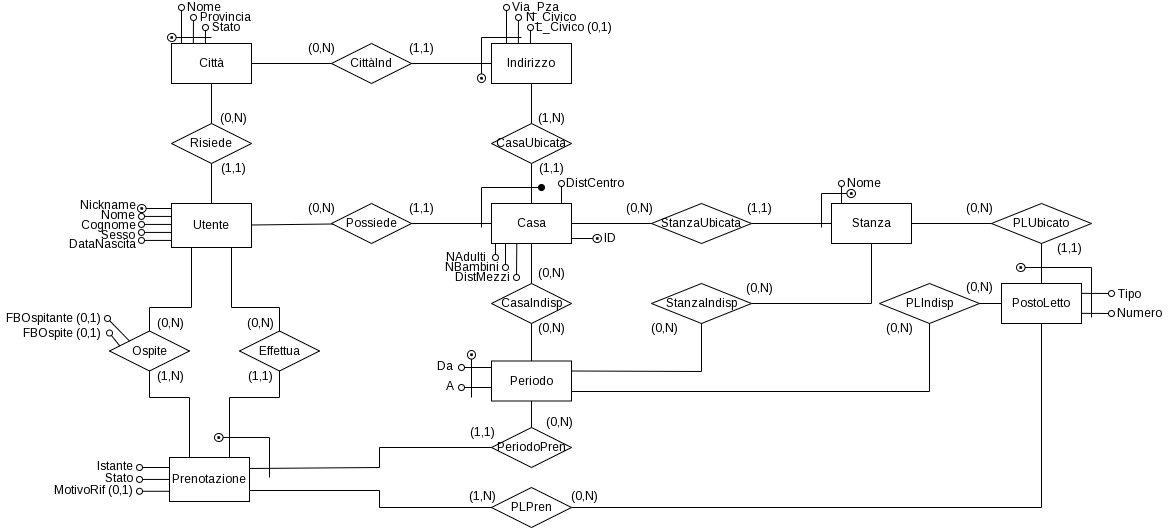
\includegraphics[width=1\textwidth]{er_ristr.png}

    \chapter{Transizione dei tipi di dati concettuali in tipi standard SQL}
      Entità Utente: \\
      \begin{tabular}{|c|c|c|}
        \hline Attributo & Tipo & Note \\
        \hline Nickname & varchar(50) & \\
        \hline Nome & varchar(30) & \\
        \hline Cognome & varchar(30) & \\
        \hline Sesso & gender\_t & \\
        \hline Nascita & datetime & \\
        \hline
      \end{tabular} \\
      \vspace{24pt} \\
      Entità Città: \\
      \begin{tabular}{|c|c|c|}
        \hline Attributo & Tipo & Note \\
        \hline Nome & varchar(30) & \\
        \hline Provincia & varchar(20) & \\
        \hline Stato & varchar(20) & \\
        \hline
      \end{tabular} \\
      \vspace{24pt} \\
      Entità Indirizzo: \\
      \begin{tabular}{|c|c|c|}
        \hline Attributo & Tipo & Note \\
        \hline Via\_Pza & varchar(50) & \\
        \hline N\_Civico & int\_nonneg & 0 indica SNC \\
        \hline L\_Civico(0,1) & char(1) & Lettera del numero civico (opzionale) \\
        \hline
      \end{tabular} \\
      \vspace{24pt} \\
      Entità Casa: \\
      \begin{tabular}{|c|c|c|}
        \hline Attributo & Tipo & Note \\
        \hline ID & int\_pos & ID incrmentale univoco introdotto per motivi di performance \\
        \hline DistMezzi & int\_pos & Distanza in metri dalla stazione dei trasporti pubblici più vicina \\
        \hline DistCentro & int\_pos & Distanza in metri dal centro città \\
        \hline NAdulti & int\_nonneg & Adulti residenti \\
        \hline NBambini & int\_nonneg & Bambini residenti \\
        \hline
      \end{tabular} \\
      \vspace{24pt} \\
      Entità Periodo: \\
      \begin{tabular}{|c|c|c|}
        \hline Attributo & Tipo & Note \\
        \hline Da & datetime & Inizio del periodo di tempo \\
        \hline A & datetime & Fine del periodo di tempo \\
        \hline
      \end{tabular} \\
      \newpage
      Entità Stanza: \\
      \begin{tabular}{|c|c|c|}
        \hline Attributo & Tipo & Note \\
        \hline Nome & varchar(20) & \\
        \hline
      \end{tabular} \\
      \vspace{24pt} \\
      Entità PostoLetto: \\
      \begin{tabular}{|c|p{0.4\textwidth}|p{0.4\textwidth}|}
        \hline Attributo & Tipo & Note \\
        \hline Numero & int\_nonneg & Un numero incrementale per identificare i posti letto dello stesso tipo in una stanza \\
        \hline Tipo & sist\_t & Il tipo identifica anche il numero di posti \\
        \hline
      \end{tabular} \\
      \vspace{24pt} \\
      Entità Prenotazione: \\
      \begin{tabular}{|c|p{0.4\textwidth}|p{0.4\textwidth}|}
        \hline Attributo & Tipo & Note \\
        \hline Istante & datetime & Istante della prenotazione, utilizzato per impedire agli utenti di effettuare prenotazioni in mancanza di feedback relativi a vecchie prenotazioni \\
        \hline Stato & pstatus & Stato della prenotazione (accettata, rifiutata, in attesa) \\
        \hline MotivoRif(0,1) & varchar(100) & Motivo del rifiuto (se la prenotazione è stata rifiutata) \\
        \hline
      \end{tabular} \\
      \vspace{24pt} \\
      Relazione Ospite: \\
      \begin{tabular}{|c|c|c|}
        \hline Attributo & Tipo & Note \\
        \hline FBOspite(0,1) & rate\_t & Feedback espresso dall'ospitante sull'ospite \\
        \hline FBOspitante(0,1) & rate\_t & Feedback espresso dall'ospite sull'ospitante \\
        \hline
      \end{tabular} \\

      \vspace{24pt}
      \large Vincoli esterni: \\
      \normalsize
      V.Indirizzo.lettera: $\forall i \;\; Indirizzo(i) \; \wedge \; NCivico(i, 0) \; \rightarrow \; \neg \exists \; l \;\; lettera(l) \; \wedge \; LCivico(i, l)$ \\
      V.Periodo.nonneg: $\forall p,i,f \;\; Periodo(p) \; \wedge \; Da(p, i) \; \wedge A(p, f) \; \rightarrow \; i \; \leq \; f$ \\
      V.Utente.fb\_obbligatorio: $\forall u,p,i \;\; Utente(u) \; \wedge \; Prenotazione(p) \; \wedge \; Istante(p, i) \; \wedge \; Ospite(u, p) \; \rightarrow \forall p',i' \; [Prenotazione(p') \; \wedge \; Istante(p', i') \; \wedge \; i' < i] \; \rightarrow \; \exists \; f \; "intero[0,5]"(f) \; \wedge \; FBOspitante(u, p', f)$ \\
      V.Effettua.ospite: $\forall u,p \;\; Utente(u) \; \wedge \; Effettua(u, p) \; \rightarrow \; Ospite(u, p)$ \\
      V.Prenotazione.motivazione\_obbligatoria: $\forall p,m \; Prenotazione(p) \; \wedge \; Stato(p, $'r'$) \; \wedge \; MotivoRif(p, m) \; \rightarrow \; m \neq NULL$ \\

      \section*{Tipi di dati personalizzati}
      \begin{itemize}
        \item gender\_t: \texttt{enum('m', 'f')}
        \item int\_nonneg: \texttt{integer check value >= 0}
        \item int\_pos: \texttt{integer check value > 0}
        \item sist\_t: \texttt{enum('Letto singolo', 'Letto matrimoniale', 'Divano letto')}
        \item pstatus: \texttt{enum('a', 'r', 'p')}
        \item rate\_t: \texttt{integer check value between 0 and 5}
      \end{itemize}

    \chapter*{Schema concettuale}
      Utente(\underline{Nickname}: varchar(50), Nome: varchar(30), Cognome: varchar(30), Sesso: gender\_t, \\
      \hspace*{2cm} Nascita: datetime, Citta: varchar(30), Prov: varchar(20), Stato: varchar(20)) \\
      \hspace*{1cm} Vincolo foreign key: (Citta, Prov, Stato) references Citta(Nome, Provincia, Stato) \\
      \hspace*{1cm} Vincolo ennupla: (CURRENT\_DATE - Nascita) $\leq$ interval('18 years') \\ \\
  
      \hspace*{-0.75cm}
      Citta(\underline{Nome}: varchar(30), \underline{Prov}: varchar(20), \underline{Stato}: varchar(20)) \\ \\

      \hspace*{-0.75cm}
      Casa(\underline{ID}: int\_pos, Proprietario: varchar(50), Via\_Pza: varchar(50), N\_Civico: int\_nonneg, Citta: varchar(30), \\
      \hspace*{2cm}Prov: varchar(20), Stato: varchar(20), NAdulti: int\_nonneg, NBambini: int\_nonneg, \\
      \hspace*{2cm}DistCentro: int\_pos, Dist\_mezzi: int\_pos) \\
      \hspace*{1cm} Vincolo foreign key: Proprietario references Utente(Nickname) \\
      \hspace*{1cm} Vincolo foreign key: (Via\_Pza, N\_Civico, Citta, Prov, Stato) references \\
      \hspace*{2cm}Indirizzo(Via\_Pza, N\_Civico, Citta, Prov, Stato) \\
      \hspace*{1cm} Vincolo chiave: (Proprietario, Via\_Pza, N\_Civico, Citta, Prov, Stato) \\ \\

      \hspace*{-0.75cm}
      Indirizzo(\underline{Via\_Pza}: varchar(50), \underline{N\_Civico}: int\_nonneg, \underline{Citta}: varchar(30), \underline{Prov}: varchar(20), \\
      \hspace*{2cm}\underline{Stato}: varchar(20), L\_Civico*: char(1)) \\
      \hspace*{1cm} Vincolo foreign key: (Citta, Prov, Stato) references Citta(Nome, Provincia Stato) \\ \\

      \hspace*{-0.75cm}
      Stanza(\underline{Casa}: int\_pos, \underline{Nome}: varchar(20)) \\
      \hspace*{1cm} Vincolo foreign key: Casa references Casa(ID) \\ \\

      \hspace*{-0.75cm}
      PostoLetto(\underline{Casa}: int\_pos, \underline{Stanza}: int\_pos, \underline{Numero}: int\_nonneg, \underline{Tipo}: sist\_t) \\
      \hspace*{1cm} Vincolo foreign key: (Casa, Stanza) references Stanza(Casa, Nome) \\ \\

      \hspace*{-0.75cm}
      Periodo(\underline{Da}: datetime, \underline{A}: datetime) \\
      \hspace*{1cm} Vincolo ennupla: Da $\leq$ A \\ \\

      \hspace*{-0.75cm}
      CasaIndisp(\underline{Casa}: int\_pos, \underline{Da}: datetime, \underline{A}: datetime) \\
      \hspace*{1cm} Vincolo foreign key: Casa references Casa(ID) \\
      \hspace*{1cm} Vincolo foreign key: (Da, A) references Periodo(Da, A) \\ \\

      \hspace*{-0.75cm}
      StanzaIndisp(\underline{Casa}: int\_pos, \underline{Stanza}: varchar(20), \underline{Da}: datetime, \underline{A}: datetime) \\
      \hspace*{1cm} Vincolo foreign key: (Casa, Stanza) references Stanza(Casa, Nome) \\
      \hspace*{1cm} Vincolo foreign key: (Da, A) references Periodo(Da, A) \\ \\

      \hspace*{-0.75cm}
      PLIndisp(\underline{Casa}: int\_pos, \underline{Stanza}: varchar(20), \underline{NPL}: int\_nonneg, \underline{TPL}: sist\_t, \\
      \hspace*{2cm}\underline{Da}: datetime, \underline{A}: datetime) \\
      \hspace*{1cm} Vincolo foreign key: (Casa, Stanza, NPL, TPL) references \\
      \hspace*{2cm}PostoLetto(Casa, Stanza, Numero, Tipo) \\
      \hspace*{1cm} Vincolo foreign key: (Da, A) references Periodo(Da, A) \\ \\

      \hspace*{-0.75cm}
      Prenotazione(\underline{Resp}: varchar(50), \underline{Da}: datetime, \underline{A}: datetime, Istante: datetime, Stato: pstatus, \\
      \hspace*{2cm}MotivoRif*: varchar(100)) \\
      \hspace*{1cm} Vincolo foreign key: Resp references Utente(Nickname) \\
      \hspace*{1cm} Vincolo foreign key: (Da, A) references Periodo(Da, A) \\
      \hspace*{1cm} Vincolo inclusione: (Resp, Da, A) $\subseteq$ Ospite(Resp, Da, A) \\
      \hspace*{1cm} Vincolo ennupla: istante $\leq$ CURRENT\_TIMESTAMP \\ \\

      \hspace*{-0.75cm}
      Ospite(\underline{Resp}: varchar(50), \underline{Da}: datetime, \underline{A}: datetime, \underline{Ospite}: varchar(50), FBOspite*: rate\_t, \\
      \hspace*{2cm}FBOspitante*: rate\_t) \\
      \hspace*{1cm} Vincolo foreign key: (Resp, Da, A) references Prenotazione (Resp, Da, A) \\
      \hspace*{1cm} Vincolo foreign key: Ospite references Utente(Nickname) \\ \\

      \hspace*{-0.75cm}
      PLPren(\underline{Casa}: int\_pos, \underline{Stanza}: varchar(20), \underline{NPL}: int\_nonneg, \underline{TPL}: sist\_t, \underline{Resp}: varchar(50), \\
      \hspace*{2cm}\underline{Da}: datetime, \underline{A}: datetime) \\
      \hspace*{1cm} Vincolo foreign key: (Casa, Stanza, NPL, TPL) references \\
      \hspace*{2cm}PostoLetto(Casa, Stanza, Numero, Tipo) \\
      \hspace*{1cm} Vincolo foreign key: (Resp, Da, A) references Prenotazione (Resp, Da, A) \\ \\
\end{document}
